\documentclass[11pt,a4paper]{article}
\usepackage[utf8]{inputenc}
\usepackage[french]{babel}
\usepackage[T1]{fontenc}

\usepackage{amsmath}
\usepackage{amsfonts}
\usepackage{amssymb}

\newcommand{\NomAuteur}{Fabrice BOISSIER}
\newcommand{\TitreMatiere}{Algorithmique II}
\newcommand{\NomUniv}{EPITA - Bachelor Cyber Sécurité}
\newcommand{\NiveauUniv}{CYBER1}
\newcommand{\NumGroupe}{CYBER1}
\newcommand{\AnneeUniv}{2021-2022}
\newcommand{\DateExam}{3 juin 2022}
\newcommand{\TypeExam}{Examen}
\newcommand{\TitreExam}{\TitreMatiere}
\newcommand{\DureeExam}{1h30}
\newcommand{\MyWaterMark}{\AnneeUniv} % Watermark de protection

% Ajout de mes classes & definitions
\usepackage{MetalExam} % Appelle un .sty

% "Tableau" et pas "Table"
\addto\captionsfrench{\def\tablename{Tableau}}

%%%%%%%%%%%%%%%%%%%%%%%
%Header
%%%%%%%%%%%%%%%%%%%%%%%
\lhead{\TypeExam}							%Gauche Haut
\chead{\NomUniv}							%Centre Haut
\rhead{\NumGroupe}							%Droite Haut
\lfoot{\DateExam}							%Gauche Bas
\cfoot{\thepage{} / \pageref*{LastPage}}	%Centre Bas
\rfoot{\texttt{\TitreMatiere}}				%Droite Bas

%%%%%

\usepackage{tabularx}

\newlength{\LabelWidth}%
%\setlength{\LabelWidth}{1.3in}%
\setlength{\LabelWidth}{1cm}%
%\settowidth{\LabelWidth}{Employee E-mail:}%  Specify the widest text here.

% Optional first parameter here specifies the alignment of
% the text within the \makebox.  Default is [l] for left
% alignment. Other options are [r] and [c] for right and center
\newcommand*{\AdjustSize}[2][l]{\makebox[\LabelWidth][#1]{#2}}%


\definecolor{mGreen}{rgb}{0,0.6,0}
\definecolor{mGray}{rgb}{0.5,0.5,0.5}
\definecolor{mPurple}{rgb}{0.58,0,0.82}
\definecolor{backgroundColour}{rgb}{0.95,0.95,0.92}

\lstdefinestyle{CStyle}{
    backgroundcolor=\color{backgroundColour},
    commentstyle=\color{mGreen},
    keywordstyle=\color{magenta},
    numberstyle=\tiny\color{mGray},
    stringstyle=\color{mPurple},
    basicstyle=\footnotesize,
    breakatwhitespace=false,
    breaklines=true,
    captionpos=b,
    keepspaces=true,
    numbers=left,
    numbersep=5pt,
    showspaces=false,
    showstringspaces=false,
    showtabs=false,
    tabsize=2,
    language=C
}


\hyphenation{op-tical net-works SIGKILL}


\begin{document}

%\MakeExamTitleDuree     % Pour afficher la duree
\MakeExamTitle                   % Ne pas afficher la duree

%% \MakeStudentName    %% A reutiliser sur chaque nouvelle page

\bigskip
\bigskip

Vous devez respecter les consignes suivantes, sous peine de 0 :

\begin{itemize}
\item Répondez sur le sujet
\item Ne détachez pas les agrafes du sujet
\item \'Ecrivez lisiblement vos réponses (si nécessaire en majuscules)
\item Ne trichez pas
\end{itemize}

\bigskip


% Questions cours files et piles
\section{Questions (5 points)}

\subsection{(1 points) \'Ecrivez l'état des deux files après avoir effectué ces opérations dans cet ordre (n'oubliez pas le(s) pointeur(s) de tête (et de queue) ) : }

\bigskip

%%%%%%%%%%%%%%%%% CENTRAGE
\vfill
\hspace{0pt}

\begin{center}

\begin{large}
enfiler 1337, enfiler 2048, défiler, défiler, enfiler 1024, défiler, enfiler 1664
\end{large}

%\vspace{2cm}

\bigskip

\begin{figure}[ht!]
\centering
\centerline{  %%% CENTRAGE HORIZONTAL
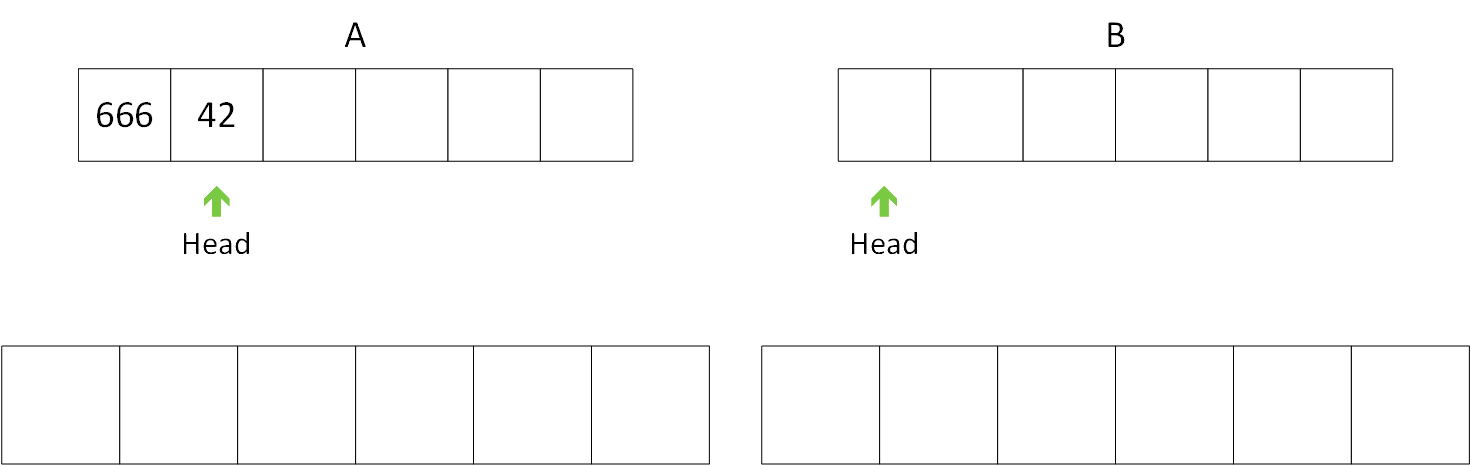
\includegraphics[scale=1]{img/Exercice1.png}
%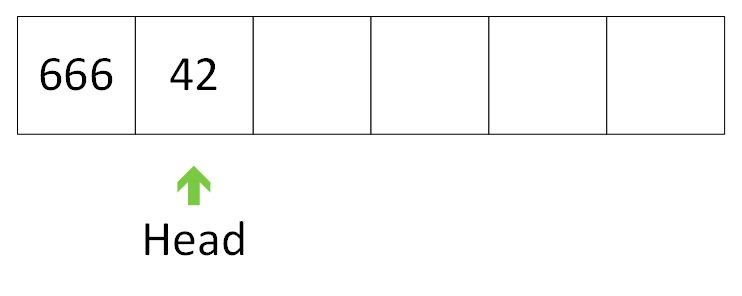
\includegraphics[scale=1,left]{img/2_elts.png}
}
%\caption{File A}
%\label{figure:1-S1-ModeleWI}
\end{figure}

\end{center}

\bigskip

%\newpage

\subsection{(0,5 point) Quel élément sortira lors du prochain \og dequeue \fg{} sur chaque file ? }

\bigskip
\bigskip

%\begin{center}
\begin{Large}
A :  \hspace{8cm}  B :
\end{Large}
%\end{center}

\bigskip
\bigskip


\subsection{(0,5 point) Quel élément sortira en dernier de chaque file ? }

\bigskip
\bigskip

%\begin{center}
\begin{Large}
A :  \hspace{8cm}  B :
\end{Large}
%\end{center}

\bigskip
\bigskip

%\vspace{5cm}

%%%%%%%%%%%%%%%%% FIN CENTRAGE

\hspace{0pt}
\vfill

\newpage

\subsection{(3 points) En admettant que l'on dispose d'une pile et que l'on insère les données \og 1 2 3 4 5 6 \fg{} dans cet ordre exclusivement, décrivez les scénarios permettant d'obtenir les sorties suivantes : }
%%% PREFERER CE TEXTE :
%\subsection{(3 points) En admettant que l'on dispose d'une pile vide et que les éléments \og 1 2 3 4 5 6 \fg{} arrivent en entrée dans cet ordre exclusivement, décrivez les scénarios permettant d'obtenir les sorties suivantes : }

\bigskip

\begin{center}
\noindent \textit{exemple : pour \og A B C \fg{} en entrée, on peut obtenir \og B C A \fg{} en sortie en faisant : \linebreak
\og push A \fg, \og push B \fg, \og pop \fg, \og push C \fg, \og pop \fg, \og pop \fg }
%%% AJOUTER CE TEXTE :
%On a bien inséré A, puis B, puis C, mais l'ordre de sortie est différent suivant les \og pop \fg}
\end{center}

\medskip


\begin{center}

\begin{large}
1, 2, 3, 6, 5, 4
\end{large}

\begin{center}
\LigneReponseTrois
% push 1, pop, push 2, pop, push 3, pop, push 4, push 5, push 6, pop, pop, pop
\end{center}


\begin{large}
2, 3, 1, 4, 6, 5
\end{large}

\begin{center}
\LigneReponseTrois
% push 1, push 2, pop, push 3, pop, pop, push 4, pop, push 5, push 6, pop, pop
\end{center}


\begin{large}
3, 5, 4, 2, 6, 1
\end{large}

\begin{center}
\LigneReponseTrois
% push 1, push 2, push 3, pop, push 4, push 5, pop, pop, pop, push 6, pop, pop
\end{center}

\end{center}


%
\section{Algorithmes (15 points)}

\subsection{(3 points) \'Ecrivez une structure de données \og \textit{my\_queue} \fg{} pouvant servir de file \textit{(la structure ne doit pas être statique)} }

\bigskip

\begin{center}
\GrilleReponseN{10}
\end{center}

\bigskip


\newpage

\subsection{(6 points) \'Ecrivez une fonction \og \textit{enqueue} \fg{} pouvant servir à enfiler un élément dans votre précédente structure \og \textit{my\_queue} \fg{} }

\bigskip

\begin{center}
%%\LigneReponseQuarante
%\LigneReponseTrente
%\LigneReponseCinq
%\LigneReponseTrois

\GrilleReponseN{24}
\end{center}

\bigskip


\newpage

\subsection{(6 points) \'Ecrivez une fonction \og \textit{dequeue} \fg{} pouvant servir à défiler un élément dans votre précédente structure \og \textit{my\_queue} \fg{} }

\bigskip

\begin{center}
\GrilleReponseN{24}
\end{center}

\bigskip


\end{document}
